\documentclass{article}
\usepackage{graphicx,fancyhdr,amsmath,amssymb,amsthm,subfigure,url,hyperref}
\usepackage[margin=1in]{geometry}
\usepackage{caption}
\usepackage{comment}
\usepackage{framed} 
\usepackage{indentfirst}
%\usepackage{supertabular,booktabs}
%\usepackage{supertabular}
%\usepackage{xtab}
\usepackage{csquotes}
\usepackage{longtable}
\usepackage{multicol}
\usepackage{appendix}
\setlength{\parindent}{1.5cm}

%------------ Algorithm Enviroment --------------
\usepackage{bbm}
\usepackage{algorithmic}
\usepackage[ruled,vlined]{algorithm2e}
%%%%%%
\SetKwProg{Fn}{Function}{}{}
%%%%%%

%------------ Bibliography  Setup --------------
\usepackage[english]{babel}
\usepackage[utf8]{inputenc}

%Includes "References" in the table of contents
\usepackage[nottoc]{tocbibind}

%------------ Hyperlinnk Setup --------------
\usepackage{hyperref}
\hypersetup{
    colorlinks=true,
    linkcolor=black,
    filecolor=magenta,      
    urlcolor=black,
    citecolor = black
}

% \hypersetup{
%     colorlinks=true,
%     linkcolor=blue,
%     filecolor=magenta,      
%     urlcolor=cyan,
% }
 
\urlstyle{same}

%--------------------------------- Tables ----------------------------------
\usepackage{multicol}
\usepackage{xtab}
\usepackage{booktabs}
\usepackage{array}
\usepackage[normalem]{ulem}
\useunder{\uline}{\ul}{}
\usepackage{floatrow}


\makeatletter
\let\mcnewpage\newpage
\newcommand{\changenewpage}{%
  \renewcommand\newpage{%
    \if@firstcolumn
      \hrule width\linewidth height0pt
      \columnbreak
    \else
      \mcnewpage
    \fi
}}
\makeatother

%----------------------- Macros and Definitions --------------------------




%%% FILL THIS OUT
\newcommand{\p}{\mathbb{P}}
\newcommand{\E}{\mathbb{E}}
%%% END
% Table float box with bottom caption, box width adjusted to content
\newfloatcommand{capbtabbox}{table}[][\FBwidth]

\newtheorem{theorem}{Theorem}



\renewcommand{\theenumi}{\bf \arabic{enumi}}

%\theoremstyle{plain}
%\newtheorem{theorem}{Theorem}
%\newtheorem{lemma}[theorem]{Lemma}

\fancypagestyle{plain}{}
\pagestyle{fancy}
\fancyhf{}
\fancyhead[RO,LE]{\sffamily\bfseries\large Stanford University}
\fancyhead[LO,RE]{\sffamily\bfseries\large CS230: Deep Learning}
%\fancyfoot[LO,RE]{\sffamily\bfseries\large \studentname: \suid @stanford.edu}
\fancyfoot[RO,LE]{\sffamily\bfseries\thepage}
\renewcommand{\headrulewidth}{1pt}
\renewcommand{\footrulewidth}{1pt}

\usepackage{float}
\usepackage{subfig}
\graphicspath{{figures/}}


%-------------------------------- Title ----------------------------------

\title{Deep Learning (CS230) Course Project Milestone}
\author{
  Persson, Samuel\\
  \texttt{joelpe@stanford.edu}
  \and
  Slottje, Andrew\\
  \texttt{slottje@stanford.edu}
  \and
  Shaw, Ian\\
  \texttt{ieshaw@stanford.edu}
}

%--------------------------------- Text ----------------------------------

\begin{document}
\maketitle

\section*{Title}
\begin{center}
 Algorithmic Trading of Cryptocurrencies Using Neural Networks
 \end{center}
\section{Introduction}

Cryptocurrencies became the talk of the financial world in 2017. With the surge of Bitcoin, Ethereum, Litecoin, and many others, everyone from institutional investors to the world's youth poured in money and interest. This relatively new asset class is just beginning to be explored by the forces of quantitative finance due to the development of data stores, established exchanges, and the increase in trading volume. Yet, this field is different than typical asset classes such as equities or fiat currencies with the dearth of regulation, no closing bells, and no friction between borders. This project seeks to explore the dynamics of this market through the lens of trading algorithms. These algorithms will capture linear and complex relationships through auto-regressive and neural network architectures. 


\section{Approach}
NEED SOME INTRO TEXT HERE
\subsection{Data}
Over the observed time horizon the examined cryptocurrencies have had relatively different price movements. Only one out of the five currencies (Etherium) had a positive return by trading Bitcoins for other cryptocurrencies at the beginning of the time frame. The exchange price between Bitcoin and other cryptocurrencies was volatile during this time horizon which is also indicated by the histogram of returns in the figure below. As expected the returns are centered around zero but has a wide distribution of returns with depreciations and appreciations as large as 15 to 20 \% during one hour of trading. 


\begin{figure}[H]
\centering
    \subfloat{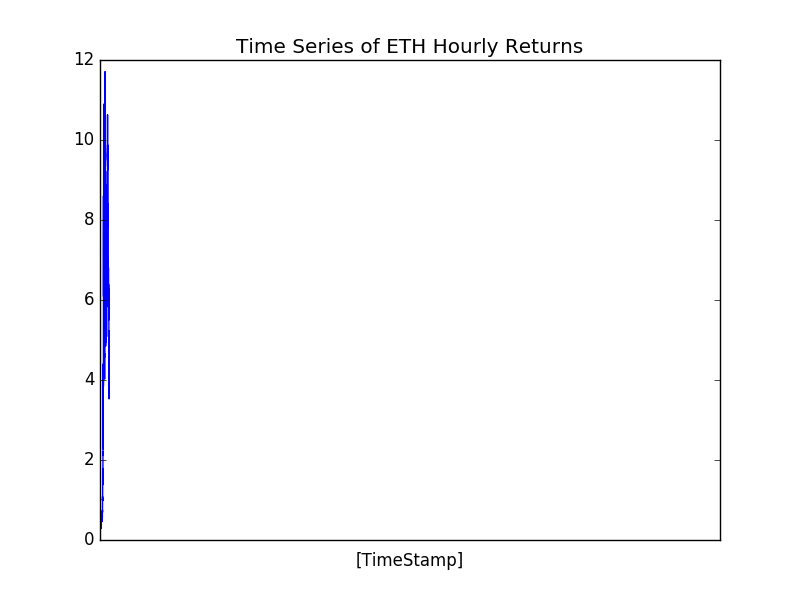
\includegraphics[width=0.45\textwidth]{ETH_ts.png}}%
    \qquad
    \subfloat{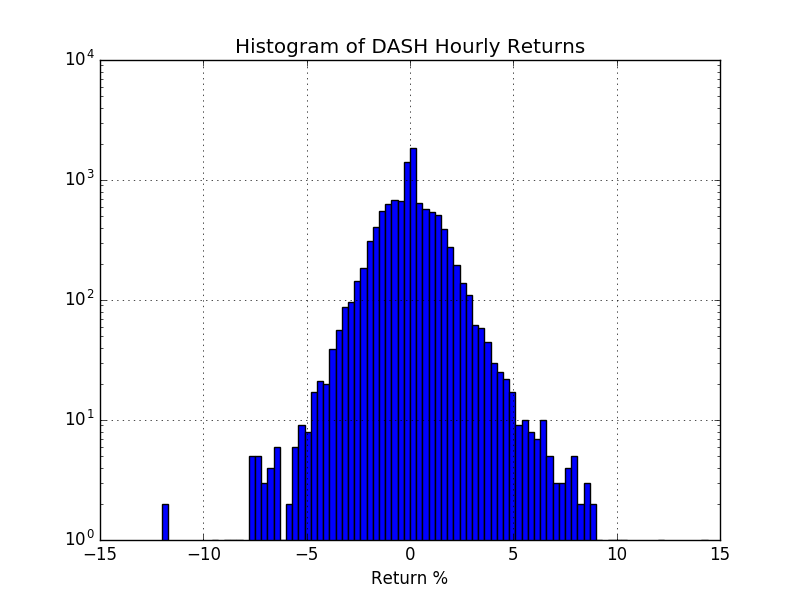
\includegraphics[width=0.45\textwidth]{DASH_hist.png}}%
    \caption{Time series of Etherium and histogram for hourly returns of DASH}
\end{figure}
\\
\\
\underline{Plots}
\begin{itemize}
\item time series
\item histogram of returns
\item performance of algo by equal allocation
\end{itemize}

\underline{Table/Metrics}
\begin{itemize}
\item sharpe
\item scorintino
\item accuracy (precision)
\item returns
\item correlation of coins
\end{itemize}

\underline{Conversation}
\begin{itemize}
\item Size of data sets; logic of splits
\item Where we got the data
\end{itemize}


\subsection{Baseline model}
To have a benchmark to compare how well the developed algorithms and models perform a baseline model was created. The strategy is simply investing an equal amount into all five cryptocurrencies and keeping them until the last hour of trading. The figure below show how the value of such a portfolio changed over time. As was indicated by the price movements of each of the individual cryptocurrencies the value change of the portfolio is as well very volatile. The benchmark values that will be used for evaluating model performance is shown in the table below. The return is slightly negative while the maximum loss of the portfolio was almost 60 \%. The Sharpe ratio relates the excess return of the strategy, i.e. how much the return exceed the risk-free interest rate, to the volatility of the strategy. Simplified, a high Sharpe ratio can be achieved by either having large portfolio returns or by having a portfolio exposed to small amounts of risk.

\begin{figure}[H]
\begin{floatrow}
\ffigbox{%
    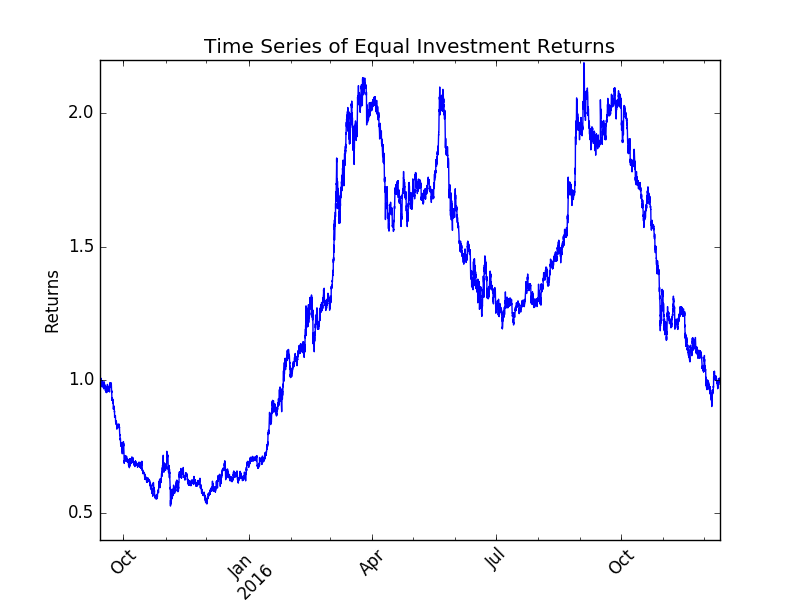
\includegraphics[width=0.55\textwidth]{baseline_ts.png}%
}{%
    \caption{Value change of baseline model}%
}
\capbtabbox{%
  \begin{tabular}{ll}
    {\ul Metric}     & {\ul Value} \\
    Return           & - 1.6 \%    \\
    Maximum drawdown & 58.9 \%     \\
    Sharpe ratio     & -0.03316   
\end{tabular}
}{%
  \caption{Evaluation of baseline model}%
}
\end{floatrow}
\end{figure}



\subsection{VAR}

\underline{Plots}
\begin{itemize}
\item loss function by epoch
\item Basic algo performance 
\end{itemize}

\underline{Table/Metrics}
\begin{itemize}
\item sharpe
\item scorintino
\item accuracy (precision)
\item returns
\item training time
\end{itemize}

\subsection{VARIMA}

% \underline{Plots}
% \begin{itemize}
% \item loss function by epoch
% \end{itemize}

% \underline{Table/Metrics}
% \begin{itemize}
% \item loss function by epoch
% \end{itemize}

% \underline{Conversation}
% \begin{itemize}
% \item loss function by epoch
% \end{itemize}

\subsection{RNN}

\underline{Plots}
\begin{itemize}
\item loss function by epoch
\item Basic algo performance 
\end{itemize}

\underline{Table/Metrics}
\begin{itemize}
\item sharpe
\item scorintino
\item accuracy (precision)
\item returns
\item training time
\end{itemize}

% \underline{Conversation}
% \begin{itemize}
% \item loss function by epoch
% \end{itemize}

\subsection{R2N2}


\underline{Plots}
\begin{itemize}
\item loss function by epoch
\item Basic algo performance 
\end{itemize}

\underline{Table/Metrics}
\begin{itemize}
\item sharpe
\item scorintino
\item accuracy (precision)
\item returns
\item training time
\end{itemize}

% \underline{Conversation}
% \begin{itemize}
% \item loss function by epoch
% \end{itemize}

\subsection{Division of labor}

\underline{Conversation}
\begin{itemize}
\item Who did what
\end{itemize}

\subsection{Work Moving Forward}

% \underline{Plots}
% \begin{itemize}
% \item loss function by epoch
% \end{itemize}

% \underline{Table/Metrics}
% \begin{itemize}
% \item loss function by epoch
% \end{itemize}

\underline{Conversation}
\begin{itemize}
\item Overfitting to training?
\item Who did what
\item exploring other loss functions?
\end{itemize}

\subsection{Future Project Ideas}

\underline{Conversation}
\begin{itemize}
\item Many ideas for future projects that have already come up
\end{itemize}

\section{Plots}
\begin{figure}[H]
\centering
    \subfloat[first]{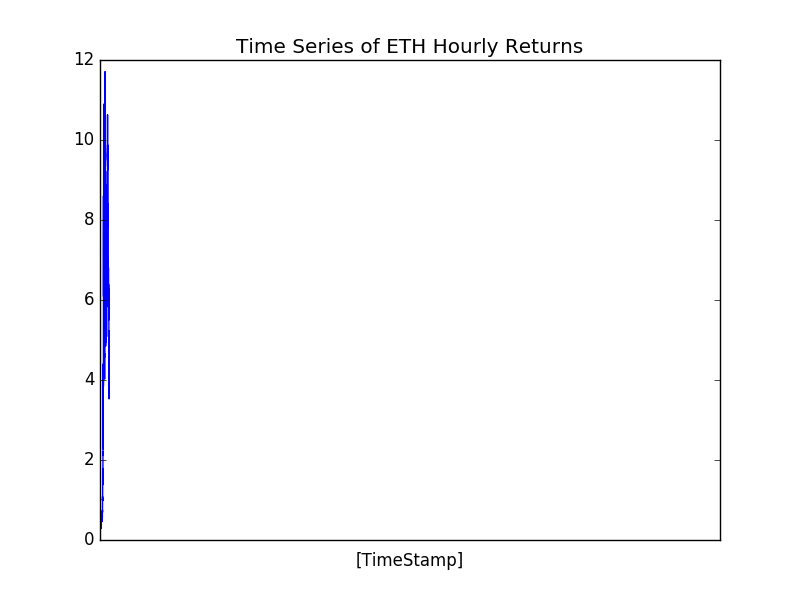
\includegraphics[width=0.45\textwidth]{ETH_ts.png}
    }
    
    \subfloat[second]{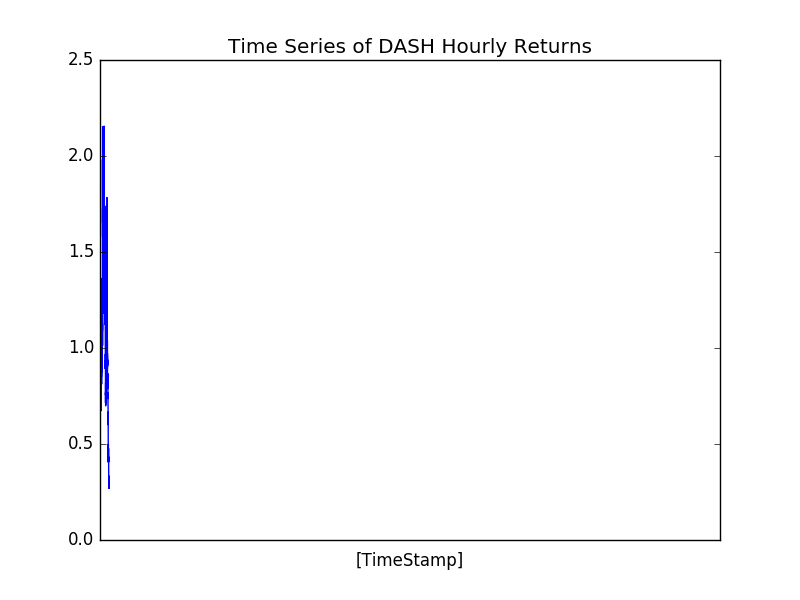
\includegraphics[width=0.45\textwidth]{DASH_ts.png}
    }
    \hspace{0mm}
    \subfloat[third]{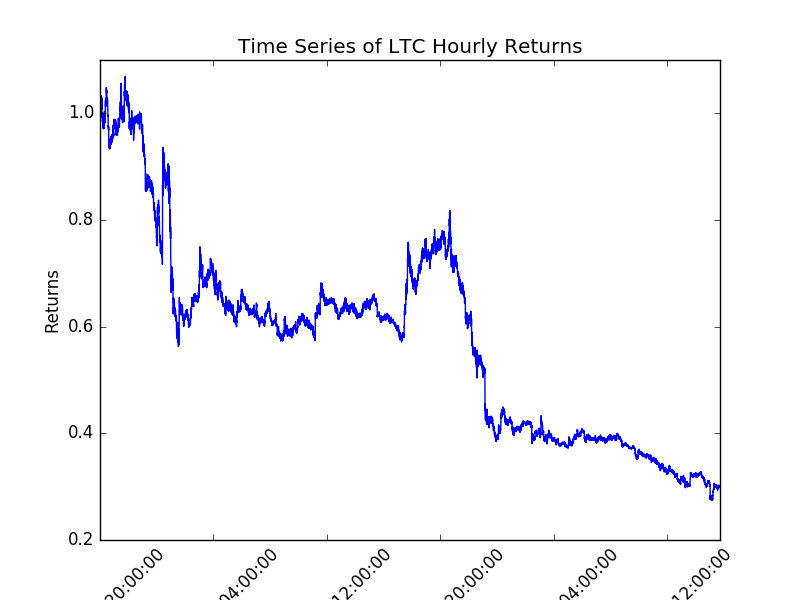
\includegraphics[width=0.45\textwidth]{LTC_ts.png}
    }

    \subfloat[forth]{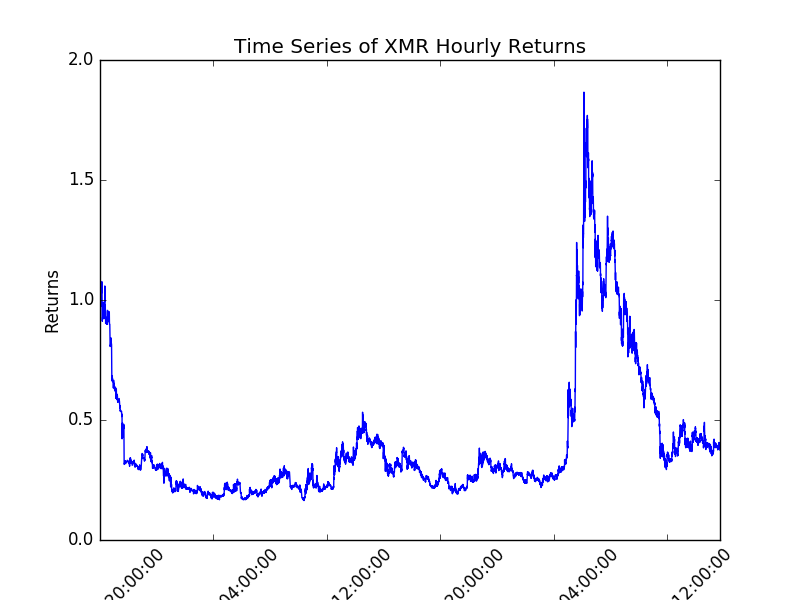
\includegraphics[width=0.45\textwidth]{XMR_ts.png}
    }
    \hspace{0mm}
    \subfloat[fifth]{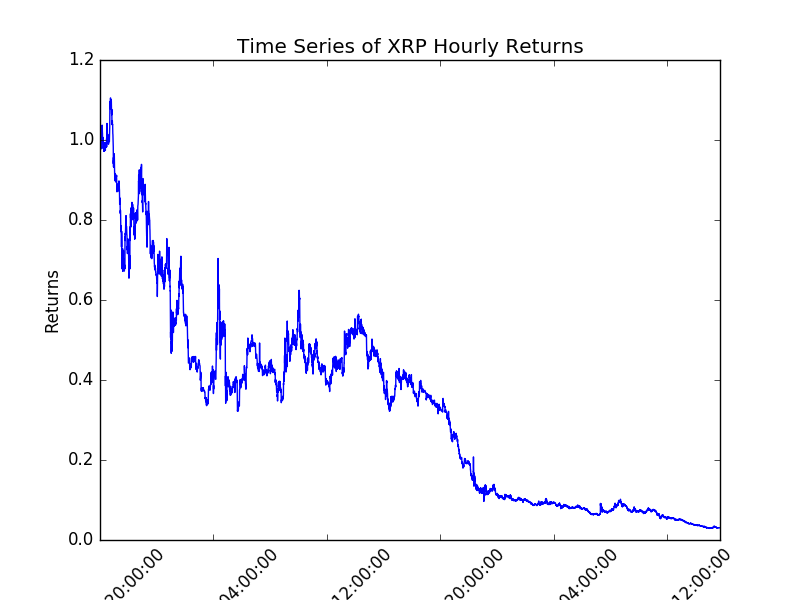
\includegraphics[width=0.45\textwidth]{XRP_ts.png}
    }
    \caption{Time series of cryptocurrencies}
\end{figure}

\begin{figure}[H]
\centering
    \subfloat[first]{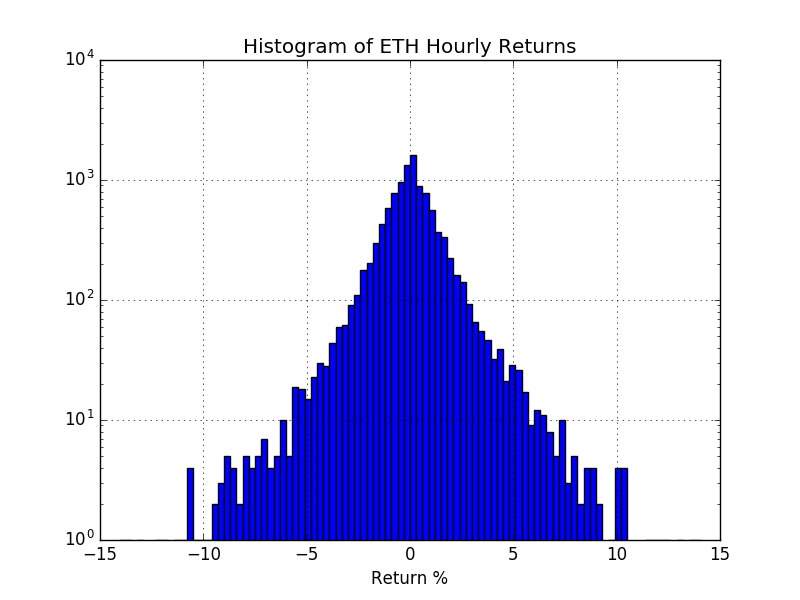
\includegraphics[width=0.45\textwidth]{ETH_hist.png}
    }
    
    \subfloat[second]{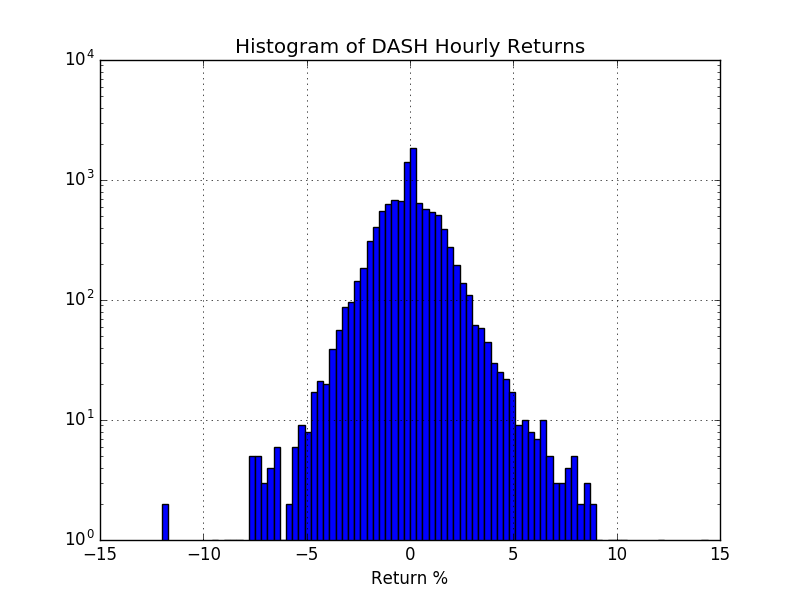
\includegraphics[width=0.45\textwidth]{DASH_hist.png}
    }
    \hspace{0mm}
    \subfloat[third]{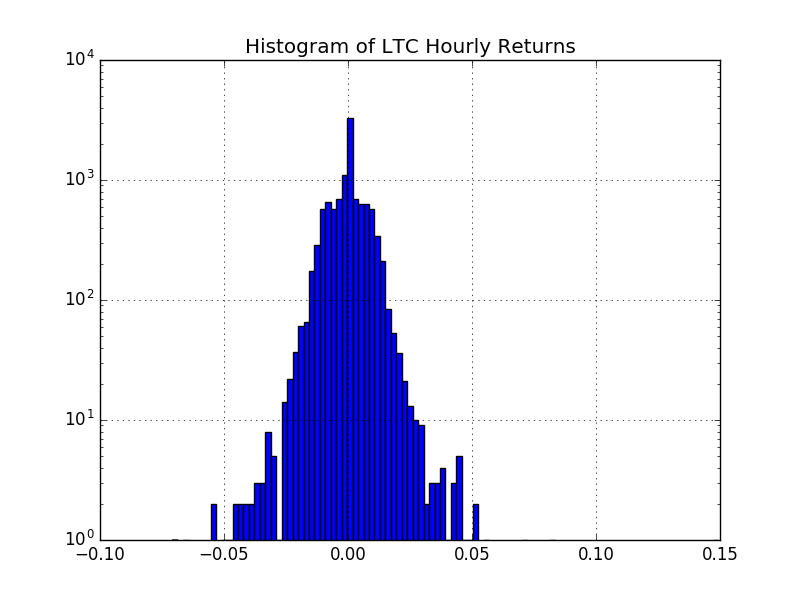
\includegraphics[width=0.45\textwidth]{LTC_hist.png}
    }

    \subfloat[forth]{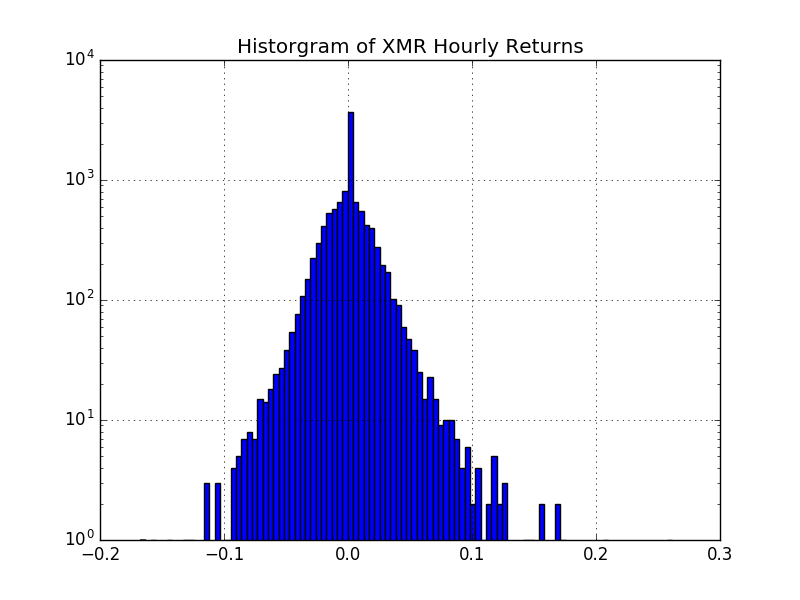
\includegraphics[width=0.45\textwidth]{XMR_hist.png}
    }
    \hspace{0mm}
    \subfloat[fifth]{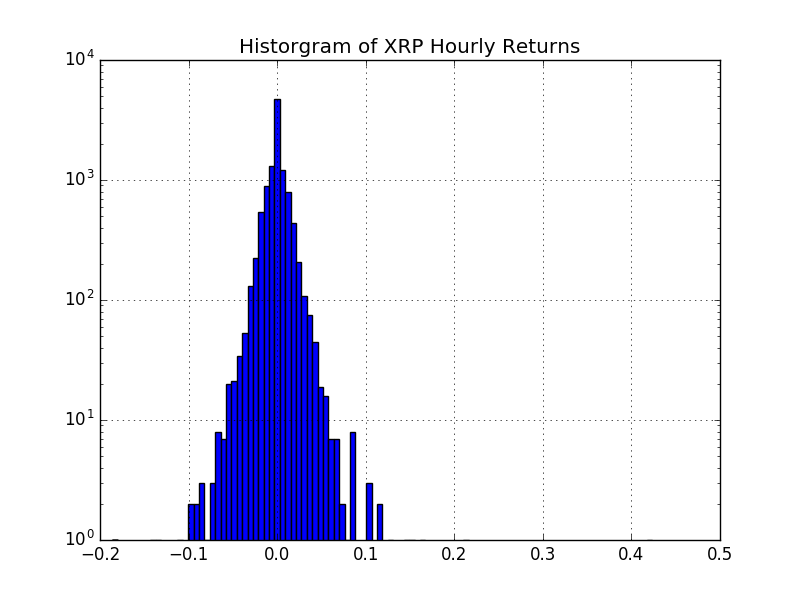
\includegraphics[width=0.45\textwidth]{XRP_hist.png}
    }
    \caption{Histogram of hourly returns}
\end{figure}

\bibliographystyle{unsrt}
\bibliography{refs}
\end{document}